\subsection{HA Napoleon}

\begin{center}
    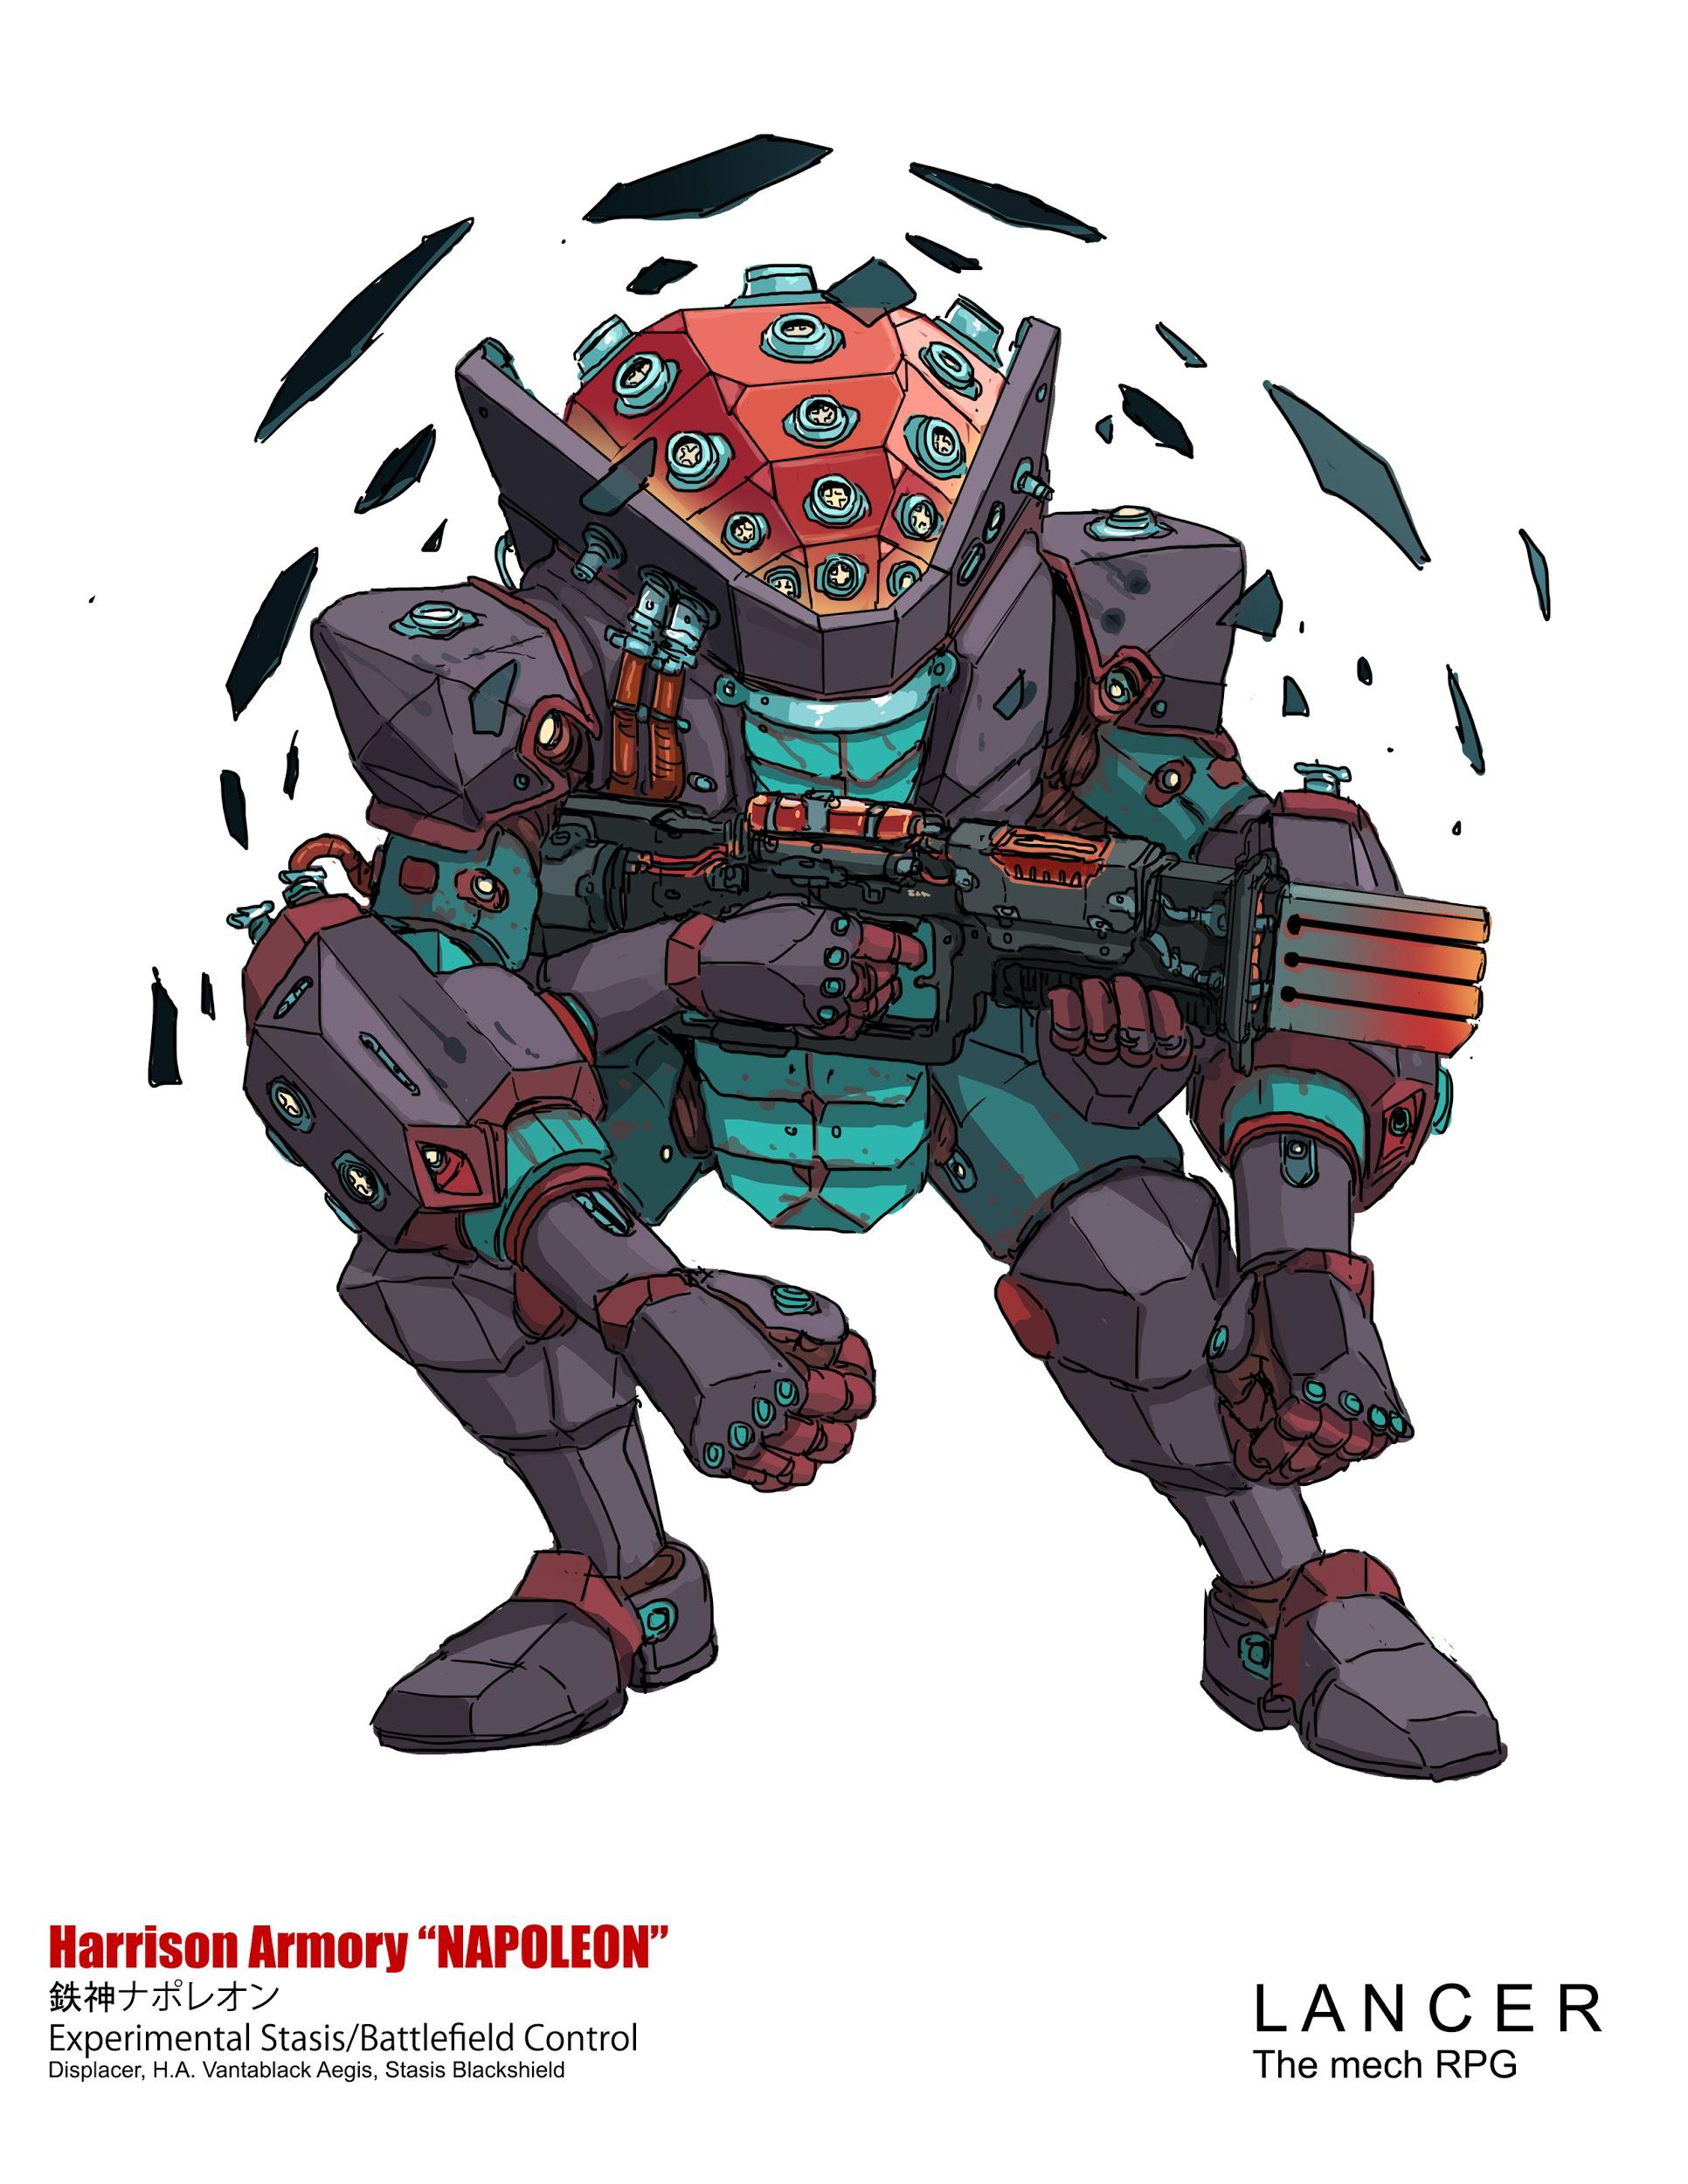
\includegraphics{Napoleon}
\end{center}

                             HARRISON ARMORY NAPOLEON

Perhaps in a tongue-in-cheek nod to its namesake, the NAPOLEON is a squat silhouette when fielded next

to other Harrison Armory chassis. But packed into its compact frame are marvels of Armory engineering,
technology that demands the NAPOLEON be piloted only by the best and the brightest. Stasis technology
is the very cutting edge of gravitic manipulation technology, only now hitting the commercial market for

those with the requisite licenses. The NAPOLEON incorporates a mix of gravitic manipulation technology,
proven anti-kinetic/energy shielding, and superpositional force multiplication to dominate enemies --
earning its namesake through battlefield success as well as stature.

                                                  License:

I. Phasing Weapon, Stasis Barrier

II. NAPOLEON FRAME, Stasis Mine, Dispersal Shield

III. H.A. Blackshield, Displacer


                                               NAPOLEON

 HP: 6          Evasion: 8                           Speed: 4           Heat Cap: 8       Sensors:  5

 Armor: 2       E-Defense: 8                         Size: 1/2          Repair Cap: 3     Tech Attack:
                                                                                          +0

                                                  TRAITS:

 Well shielded: If the NAPOLEON would take half damage from an effect (weapon, system, explosion,
 etc) on a successful check of any kind, it instead takes 0 damage.

 Flash Aegis: When the NAPOLEON Braces, it reduces damage to 0 instead of gaining resistance

                                            SYSTEM POINTS: 7

                                                 MOUNTS:

 Main/Aux Mount

                                               CORE system




                                                HA Vantablack Aegis

 The Armory’s VANTAblack AEGIS system is a breakthrough in personal shielding developed by HA’s
 Think Tank. In line with other NHP-derived technologies, the VANTAblack is a so-called “black-box”
 technology; pilots with requisition power to obtain a VANTAblack system are typically of high rank or
 standing within HA, and the inner workings of the system are not known to the public at large. On
 outward appearance, the VANTAblack system has been described by Cosmopolitan pilots as similar to
 the void/blindness one has when looking out at blinkspace; it is safe to assume that the system utilizes
 unstable blinkfield technology to manifest a thin blinkspace bubble within defined parameters around
 the system -- the blinkfield can only sustain for a brief moment, but can be flickered to create an
 essential-total blinkspace dome.

 Active (requires 1 core power): Activate Aegis
 Quick Action

 A shimmering, utterly black field envelops your mech, covering it like a second skin, and taking only a
 few moments to activate. While this field is active, your mech reduces all damage from any source to 1
 (after armor as normal), though it can still be grabbed, knocked back, pinned, thrown, and affected by
 other mechs.


 While this shield is active, your mech can only move and make the grapple, improvised attack, ram,
 and boost actions. It cannot take free actions, reactions, or overcharge, and cannot use any systems or
 benefit from Flight (if it’s already flying, it falls). It cannot make or be the target of any tech actions
 (including lock on, etc), cannot benefit from beneficial tech actions (such as lock on, bolster, etc) and
 cannot communicate or receive communications with or from anyone except the GM (though hand
 signals are still possible).


  It can still be affected by statuses, grappled, and take heat. It can otherwise interact normally with the
 world, such as picking up or dragging items, etc.


 The shield lasts until the end of the current challenge, or about ten minutes otherwise.

 Damage that goes through reduction (such as paracausal ammo) can still harm the Napoleon while its
 aegis is up.

Phasing weapon

Phase-Ready ammunition, as first described after its incorporation into the civil hostilities on Luna de Oro,
is the “devil‘s round“: each round contains a nanoprocessor suite networked with its firing weapon that,
ideally, calculates and translates the specific nature of that round‘s superpositional relation with its

doppelgänger in the immediate space before its intended target. To wit, Phase Ready ammunition, when
fired, exists in two places at once: exiting the barrel of the weapon it was fired from, and at the moment of
impact into its target. The prime round may never hit its target, but as it already exists at the moment of

impact, its doppelgänger round will hit its target. The fuzzy nature of such spooky action occurs in a way
not fully understood save for in the faltering explanations of Harrison Armory‘s NHP Think Tank; as such,
the action is not perfect, but falls within acceptable parameters for licensed production.

2 SP

Mod

Choose 1 weapon. This weapon can totally ignore line of sight and cover as long as you roughly
know your target’s location when you attack, but your target counts as having invisibility if you




attack this way. This weapon can attack through solid walls or obstacles, as long as its target’s
location is known and they are in range.


Stasis Barrier

Stasis Barriers are the result of Harrison Armory‘s interest in gravitic manipulation and superpositional
negotiation. Contained within a solid-state generator/projector, a Stasis Barrier is a deplorable wall of

antigravity, contained by its power supply, that interdicts and denies most all incoming kinetic and energy-
based weaponry. Another of HA‘s NHP Think Tank development, the Stasis Barrier is now a mainstay of the
Armory‘s personal and materiel defense line and a common enough sight on all Armory Depot/

Development worlds. By manipulating local gravitational forces, the Barrier rejects projectiles and energy
lances, denying particles and waves both on a molecular level; matter that impacts a Stasis Barrier simply

ceases to exist, save for anomalous fluctuations that cause some projectiles to break through. As the
Barrier is technology from the Armory‘s Think Tank line, some of its fuzzy nature is not fully understood, but
rest assured failsafes have been installed to force a regular cessation of projection to ensure the device

remains operating within established safe parameters.

2 SP, Limited (1)

Shield, Deployable
This module deploys as a 4 space long piece of size 2 cover that lasts until the end of the current
challenge. While behind the barrier, a target counts as having heavy cover and has resistance to
all damage from blast, line, and cone attacks. At the end of the challenge, it deactivates and is
used up. The cover itself is immune to all damage.


Stasis Mine

Stasis Mines developed by the Armory‘s NHP Think Tank, are portable, unit-specific versions of Stasis

Barriers. Initially pegged as a potential personal shielding device, early tests proved that stasis is as-yet
detrimental to the individual inside a projected field. Think Tank suggests that the cognitive hazards of
sudden and total pause of temporal/gravitic/positional existence without preparation -- however long the

stasis session lasts -- is irrevocably traumatic.

1 SP,  Limited (1)


Mine

You can detonate this mine with a quick action once planted (or it activates normally). Once
detonated, this mine creates a burst 4 area around it. Affected targets may make an agility check
with 1 difficulty to escape if on the edge, otherwise they are trapped inside. The area inside is
locked from the normal flow of space time, creating an impermeable barrier around its edge.
Effects, mechs, and pilots inside are stunned and removed from play until the end of next round,
and all other effects cannot penetrate into the area. Time does not flow normally for targets
inside the area (it stops completely), and is separate to the outside world. Active effects, attacks,
modules, and other individuals and actions inside the area pause. At the end of the the next
round (after all characters have acted), this area returns and resumes play as normal.


Dispersal Shield

Dispersal Shielding is a milder form of stasis projection that manipulates only gravity, adjusting the
perceived mass of its user so that projectiles and excited particles bend and warp around and through




them. Hostile fire does not quite “miss“ so much as they undergo atomic shuffling, disincorporating on the
atomic level so that they pass through their targets without colliding.

3 SP, Unique
Reaction, Shield

1/round you can force any attack that misses you to be re-rolled against a target of your choice
within your attacker’s range (even a target allied to them).


Harrison Armory Blackshield

The Armory Blackshield leans into the fuzzy nature of quantum manipulation characteristic of Think Tank
research and development. The Blackshield operates in similar fashion to blinkspace gates, generating a

pulse of spherical energy that allows its operator to pierce perceived space/time and exist, for a moment, in
the null-environment of blinkspace. Blinkspace, described by early test pilots and their NHP companions, is
a void, a space outside of human perception that it at once infinite and without form, blank and cacophony.

NHPs that accompanied those first pilots have since been retired, their handlers citing recursive ontological
tail-chasing and paracausal obsession; since then, NHP protocols have been updated to include a sense-
exposure doctrine, allowing them to do as corporeal, sapient pilots do and simply accept the unreality of

blinkspace without going mad. Think Tank NHP‘s and their counterpart engineers acknowledge the tactical
benefits of (non)momentary (non)existence in blinkspace, but they caution pilots against repeated exposure
without sufficient pre-and-post exposure conditioning and counseling.

2 SP
Shield, Unique

Full Action
4 heat (self)

As a full action, this system can be activated to generate a burst 4 area centered on user. While
active, the flow of time is altered drastically in a small sliver of space in a bubble around the user.
Nothing, not even light, can enter or exit the shield. It is impermeable and invulnerable. When the
shield is activated, mechs caught on the edge must make an agility check to choose which side
they end up on, otherwise the user chooses. To those inside the shield, the world outside the
shield goes totally black, and the inverse happens from outside. No action or effect can enter or
exit the shield while it is active or draw line of sight though (even those that normally ignore it),
though time passes normally on both sides. The shield drops automatically at the end of the
user’s next turn.


Displacer

The Displacer is the result of ongoing blinkspace exposure tests in Think Tank‘s R\&D department and
miniaturization of commonly employed interstellar travel methods. The Displacer itself is conventional in

appearance but requires a massive secondary, dorsal-mounted core in order to power: when fired, the
Displacer identifies a bubble of local space (size and location determined by the firing pilot) and snaps it
into blinkspace. Where the contents of that bubble go is unknown, but the effect is dramatic: anything

inside the projected bubble simply ceases to exist in this dimension, transported somewhere else in the
void of blinkspace. The Displacer makes no sound when fired, but the sudden and necessary venting of its




power supply is tremendous; similarly, the heat wave of its backblast is deadly to any unshielded personnel
exposed to it.

Main Rifle

Unique, Loading, AP, 10 heat (self)

Range 10, Blast 1

10 energy damage
